% THIS IS SIGPROC-SP.TEX - VERSION 3.1
% WORKS WITH V3.2SP OF ACM_PROC_ARTICLE-SP.CLS
%APRIL 2009

\documentclass{acm_proc_article-sp}

\begin{document}

\title{NV: Nessus Vulnerability Visualization for the Web}

\numberofauthors{5} 

\author{
%\alignauthor
%Lane Harrison
%       \affaddr{Oak Ridge National Lab}\\
%       \email{trovato@corporation.com}
% 2nd.
%author
}

\maketitle
\begin{abstract}

Network vulnerability is a critical component of network security. 
Yet vulnerability analysis has received relatively little attention from the security visualization community.  

\end{abstract}

% A category with the (minimum) three required fields
%\category{H.4}{Information Systems Applications}{Miscellaneous}
%A category including the fourth, optional field follows...
%\category{D.2.8}{Software Engineering}{Metrics}[complexity measures, performance measures]

%\terms{Theory}

%\keywords{ACM proceedings, \LaTeX, text tagging} % NOT required for Proceedings

%**Screen shot of overview here**
%![Alt Text](screenshots/overview.png)
\begin{figure}
  \centering
  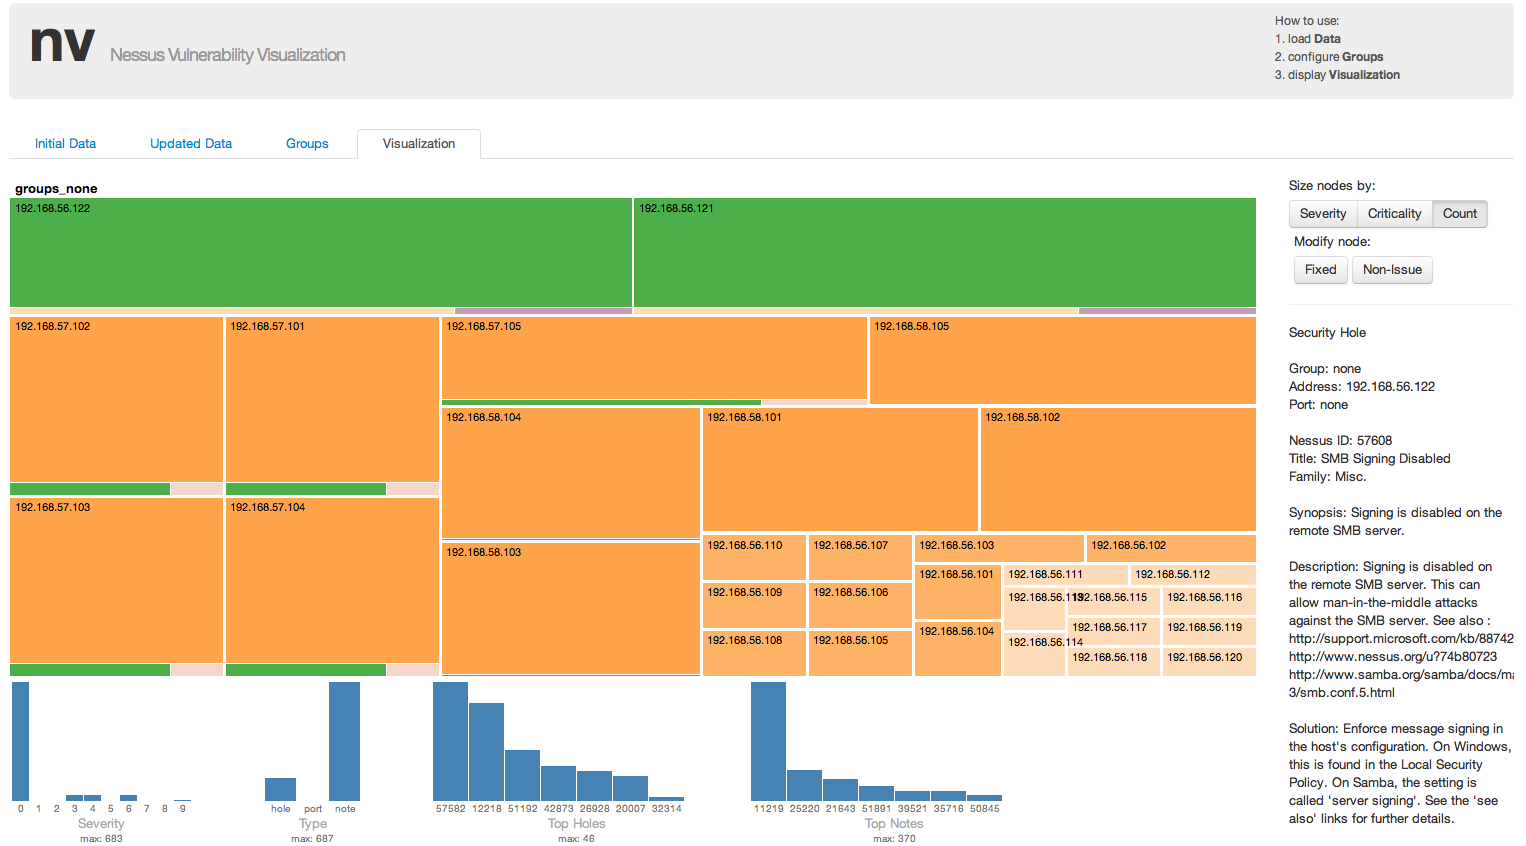
\includegraphics[width=0.5\textwidth]{../screenshots/overview}
  \caption{asdf}
\end{figure}

\section{Introduction}
In order to assess the security posture of the servers and workstations on their network, system administrators and security analysts use vulnerability assessment tools such as Nessus. Such tools probe machines to determine which network ports are open, what services are running on the ports, and, most importantly, what versions of those services are running. Identifying the services and the versions enables these tools to match them with known vulnerabilities. Nessus and similar tools can produce an overwhelming amount of data for large networks. Traditional reporting tools present the data tabularly, often with color coding to attempt to provide an overview of each vulnerability's severity. But this data can be very large with little support for comparing individual or logical groupings of machines. Further, it can be difficult to determine whether the overall vulnerability state of a network has increased or gotten worse between scans from different points in time.

Increasingly, vulnerability scanners such as Nessus are used by administrators to assess the state of their networks.  While there are many alternative tools available, Nessus is currently the most commonly used choice, and has been for some time. (Cite: sectools did surveys according to wikipedia.)  These tools generally do a very thorough job of gathering the information, but generally present it as simply a large list of individual results, which on larger networks can quickly become difficult to prioritize.

Nv intro...

Nv also allows analysts to specify logical groupings that reflect analyst's situated knowledge [cite Goodall CSCW paper]. Additionally, nv enables analysts to capture criticality scores for individual and groups of machines in their network. This information is then used by to affect size and other visual features in the treemap, which helps ensure that high-value machines receive the most attention.

Specifically, our contributions to the field of security visualization are as follows:

- A visualization tool that supports security vulnerability awareness, analysis, and tracking; and

- A framework for building web-based visualizations that do not send sensitive data to servers

In the following section, we discuss related work in vulnerability visualization and analysis. Afterwards, we discuss the design of nv. We then present several case studies involving Nessus scans from multiple systems. We conclude with a brief discussion on web-based security visualization tools and on our future plans for nv.

\section{Related Work}

Currently, most computer vulnerability analysis is done using graph-based
techniques to model the state of the system. One such technique is known as
Topological Vulnerability Analysis (TVA). TVA uses the network state and attack
vectors between machines to create an attack graph that will model all possible attack paths in a
network. To generate these attack graphs TVA uses information from scanning
tools such as Nessus and Retina. These graphs generated by TVA tend to be 
large, so it introduces an aggregation and visual analysis element to make the
models easier to comprehend by an analyst. One aggregation method used by the TVA
visualization is to aggregate machines based on their ability to access other machines. A group of
machines will be aggregated if each node in the group has access to every other
node in that group.
These groupings are then aggregated into a single node in the visualization.
**Noel** see Prole short paper from VizSec too.

Researchers have also used model checking tools like NuSMV to manipulate graph
representations of a network where each node is a state of the network and each
transition represents an exploit.  This type of attack graph allows an analyst
to focus efforts on patching exploits (edges) that create the largest
disconnects in the graph. This type of analysis is convenient because we
already have graph algorithms that can efficiently perform such analysis.
**Aman**

Ou, Govindavjhala and Appel take a different approach to security analysis in
their MulVAL project.
They attempt to model the interactions between known vulnerabilities and
software bugs, configurations and permission policies.  In their approach an
analyst will specify the system and policies in a logic language that is a subset of the
Prolog logic programming language and vulnerabilities in the Open Vulnerability
Assessment Language. After the systems, policies, and vulnerabilities are defined
the MulVAL system uses a two-phase algorithm to simulate both attacks and policy
checking. The system generates all possible attacks based on the
vulnerabilities and then compares those with the defined policies to detect
violations.
**Ou**

While these approaches provide a detailed assessment of the accessibility of vulnerable targets, our goal was to create a more widely applicable system. Nessus is the de facto standard for vulnerability assessment. Rather than build an entire system, we wanted to leverage data that is already commonly used in the security community. This approach increases the potential adoption and value to the security community. In addition to leveraging data that analysts already use to encourage adoption and use, we wanted our system to be usable without installing any software, so our approach is web-based, but does all processing of potentially sensitive data on the client within the browser.

\section{System Design}
The goal of nv is to support the sysadmin's understanding of vulnerabilities in their network by combining the results of a Nessus scan in raw format and (optionally) a list of critial machines in their network into an interactive visualization.
This visualization is designed to support common workflows in vulnerability discovery, analysis, and mitigation.
Some of these are described in the Case Studies sections.
This section covers the visualization and interaction design.

\subsection{Data}
Nessus data in detail

The Nessus scan results provide significant detail about the state of all machines on the specified network.
(TODO talk about how the scan actually works?) This information includes the port the vulnerable service is running on, what service and what version is running, what other versions of this software share this vulnerability, and a general description of the vulnerability.
These results also indicate whether this is an actual vulnerability or just a general security notice, and it also provides a severity score and several unique identifiers related to this vulnerability, which can be used to find additional information.
The results also often give information about how this vulnerability can be patched or otherwise mitigated.
Figure nnnnnnnnnnnnnnnnnnnnnnnnnnnnn (TODO) shows an example; this particular example is from the VAST Challenge 2011 data set.

%results|192.168.2|192.168.2.175|cifs (445/tcp)|46844|Security Hole|Synopsis :\n\nThe remote Windows host contains a font driver that is affected by\na privilege escalation vulnerability.\n\nDescription :\n\nThe remote Windows host contains a version of the OpenType Compact\nFont Format (CFF) Font Driver that fails to properly validate certain\ndata passed from user mode to kernel mode.\n\nBy viewing content rendered in a specially crafted CFF font, a local\nattacker may be able to exploit this vulnerability to execute \narbitrary code in kernel mode and take complete control of the \naffected system.\n\nSolution :\n\nMicrosoft has released a set of patches for Windows 2000, XP, 2003,\nVista, 2008, 7, and 2008 R2 :\n\nhttp://www.microsoft.com/technet/security/Bulletin/MS10-037.mspx\n\nRisk factor :\n\nHigh / CVSS Base Score : 9.3\n(CVSS2#AV:N/AC:M/Au:N/C:C/I:C/A:C)\n\n\nPlugin output :\n- C:\\WINDOWS\\System32\\Atmfd.dll has not been patched\n    Remote version : 5.1.2.226\n    Should be : 5.1.2.228\n\n\n\nCVE : CVE-2010-0819\nBID : 40572\nOther references : OSVDB:65217,MSFT:MS10-037\n


%it would be great if the use case section, see below for my edits, was
%reflected in the following 'visualization and interaction section'
%where each of these is discussed in turn. that would help tie the
%design to the use cases we are trying to support.

\subsection{Use Case}

% TODO Lane find where john mentions these and cite; also add to bibtex
% Goodall, John R. , Wayne G. Lutters, and Anita Komlodi. "Developing
% Expertise for Network Intrusion Detection." Information Technology &
% People 22(2), Emerald Group Publishing Limited, 2009, 92-108.
% 
% Goodall, John R., Wayne G. Lutters, and Anita Komlodi. "I Know My
% Network: Collaboration and Expertise in Intrusion Detection."
% Proceedings of the ACM Conference on Computer-Supported Cooperative
% Work (CSCW), ACM Press, 2004, 342-345.


The primary goal of nv is to support system administrators in understanding the
vulnerabilities within their network in order to support their
decision-making in determining how to allocate and prioritize their
limited resources in order to reduce the security vulnerability of
high-value targets within their network.

Specifically, the main tasks that nv seeks to support are:

- Identifying the individual machines that have the most severe vulnerabilities.
- Discovering the services that have the most vulnerabilities within
their network.
- Identifying the exposure to vulnerabilities within groups of
machines where those groupings reflect the analyst's mental model of
their network.
- Determining the high-value machines that are vulnerable to exploitation.
- Comparing point-in-time snapshots of the security state of the
machines in the network and understanding the differences between the
two points.

\subsection{Visualization and Interaction}
Nv consists of multiple coordinated views including a treemap, several histograms, and a detail-information area showing information on the selected Nessus id.
Each of these are designed to support a specific aspect of the vulnerability analysis workflow

Our primary visualization is a zoomable treemap (TODO cite).
We chose to use a treemap over other hierarchical visualization methods such as network/tree-layouts for several reasons.
First, our goal with nv is to support the analysis of Nessus scans on large networks.
While information on the network topology is useful for vulnerability analysis, it is important to note that in large dynamic networks, a complete network topology is often either unavailable or too large to be visualized directly.
The space-filling aspects of treemaps make them more scalable in this regard.

The treemap allows us to easily identify machines with the most severe vulnerabilities. The administrator's eye will be naturally drawn to the darkest-colored node in the treemap, revealing the machines with the largest amount of these severe vulnerabilites. The treemap allows the system administrator to group machines together in a way that makes sense to them personally. Often times the system administrator has a mental picture of how their network is laid out and benefit from using a flexible environment that lets them customize it as they see fit. Again, using custom grouping, the system administrator can easily group high-value machines into a single group and can be monitored closely for vulnerabilities. Allowing the administrators to compare two different points in time of their network is also crucial. They can use these snapshots to not only monitor how efficient the network is being patched but also see how many times the network has been receiving vulnerabilites over a period of time. If there are more "new" nodes than "fixed" nodes, then they can assume that either attention to that group of machines as been depleted or that the group has become more suseptible to vulneratibilies over time. All of these analyses are important to administrators and can help them to monitor and protect their network more efficiently and effectively.

Another reason we used treemaps was for their ability to effectively make use of both size and color for encoding data attributes.
Since Nessus data is not stored in a hierarchical form by default, it could be visualized using many multi-dimensional visualization techniques, such as parallel coordinates or scatterplot matrices.
However, because the scalability of the visualization was a primary concern, we opted to nest the data from individual vulnerabilities and ports up to IPs and groups of IPs.

We also use data-accumulation and coloring methods to ensure that data is not obscured by the hierarchy.
For instance, when comparing two Nessus scans, nodes are colored by the maximum count of issue states (fixed, open, or new issues) in their child nodes.
A potential disadvantage of this approach is that a node could contain sligthly more fixed issues than open issues, and yet will still be colored green.
To alleviate this problem, we add the option to split the nodes by issue-state higher in the hierarchy.
Both options are shown in figure (TODO make figure).



%**Screen shot of state_issue here**
%![Alt Text](screenshots/state_issue.png)
\begin{figure}
  \centering
  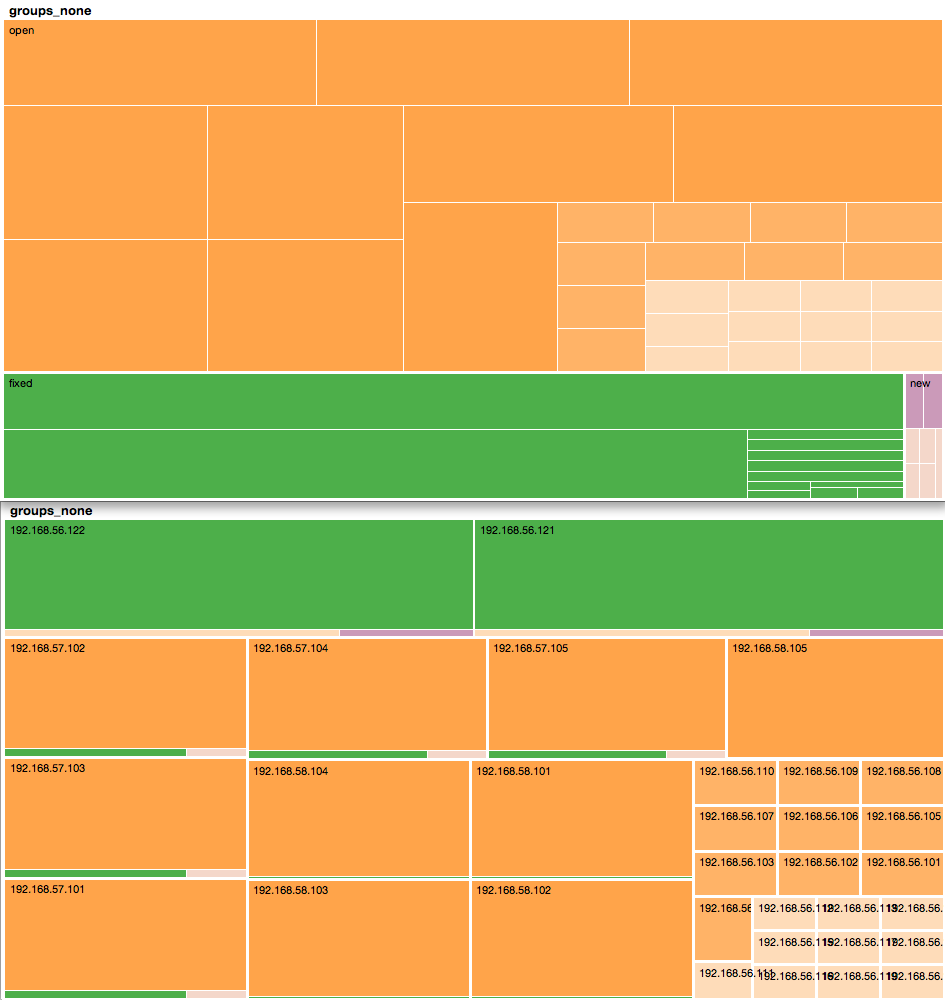
\includegraphics[width=0.5\textwidth]{../screenshots/state_issue}
  \caption{asdf}
\end{figure}

The advantage to separating issue-states higher is that the analyst can explore only the fixed issues or only the open issues.
However, the disadvantage of this approach is that the IPs are then separated since they can appear in any branch of the hierarchy (fixed, open, and new).
To our knowledge, there exists no widely accepted visual technique that can effectively represent multiple attributes at every level in a treemap.
However, we plan to explore other common approaches such as glyphs and combined color scales in future versions of nv.


Since analysts can specify the criticality of both individual machines and groups of machines in nv, the treemap includes sizing by criticality as an option.
The most critical machines therefore appear as larger nodes, while still being colored by severity.
Other sizing options include severity (the default) and by issue counts.
Dual encoding severity with both color and size can be useful, as the darkest colored and largest nodes appear at the top left in each level of the histogram.

The color scales in the treemap were created using ColorBrewer2 (TODO cite).
While the primary color scales shown in the paper are designed to have semantic meanings (green for fixed, red for new, orange for open), we also include a colorblind-safe version, which is shown in figure (TODO figure).


%**Screen shot of cb here**
%![Alt Text](screenshots/cb_version_both.png)
\begin{figure}
  \centering
  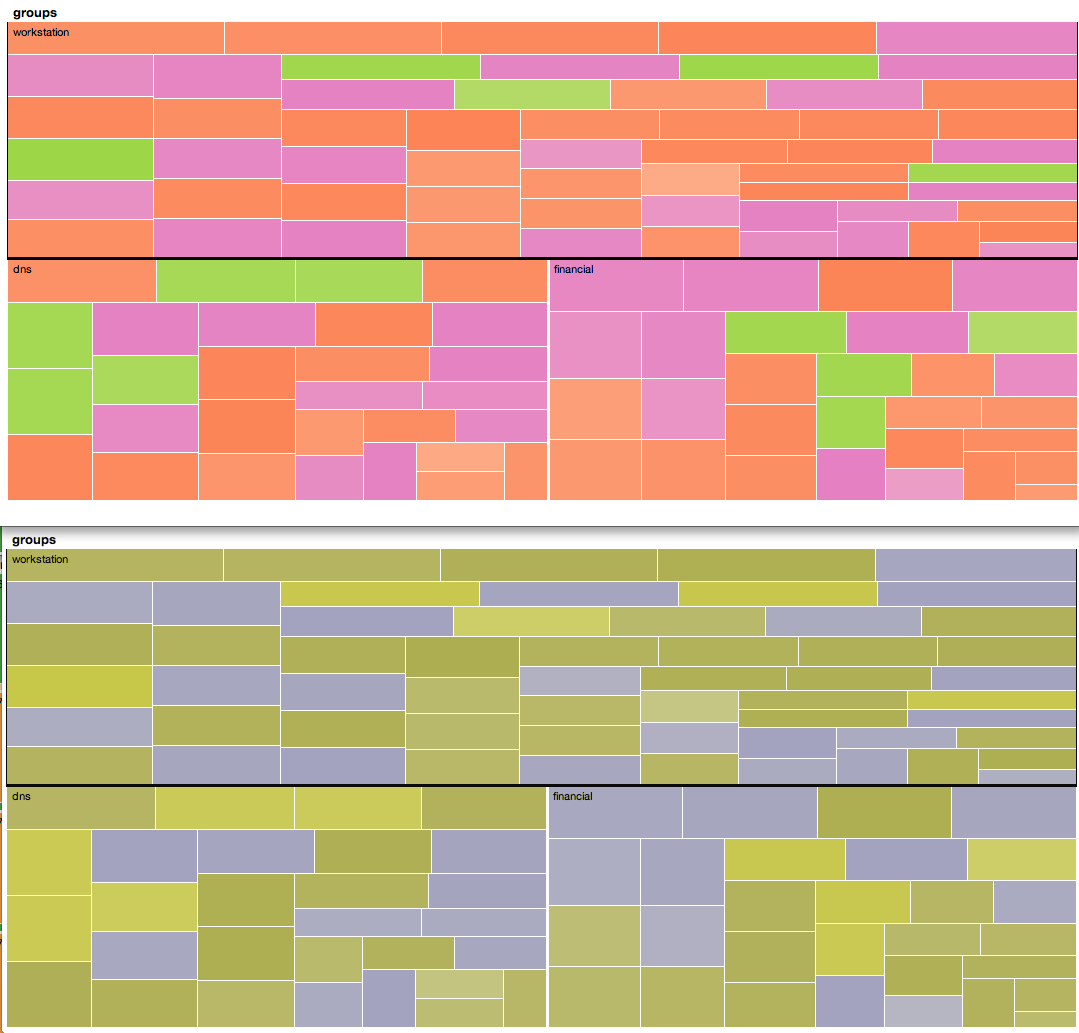
\includegraphics[width=0.5\textwidth]{../screenshots/cb_version_both}
  \caption{asdf}
\end{figure}

Nv includes several histograms, including issue-type (note, hole, or open port), severity (CVSS score), top Nessus note ids, and top Nessus hole ids.
These histograms serve dual purposes, as both overviews of the data and as filters by which sysadmins may guide their analysis.
For instance, by brushing over the highest values in the severity histogram, the appropriate nodes in the treemap are highlighted.
This works by examining each child of each element in the current level of the hierarchy.
Another use of the histograms is to easily highlight the most commonly occuring issues in the network.
A possible drawback of this approach is that sometimes the least common issues can be the most damaging.
However, this issue is mitigated by the fact that the treemap can be be sized and colored by severity, which makes the most damaging issues easy to find.
The histograms also operate in as conjunction (AND), meaning that the sysadmin can specify queries such as all issues of type hole with severity of 5 or greater.

The Nessus information area is updated when the sysadmin drills down to the level at which Nessus issue-identification numbers are shown.
The area then updates with detailed information about the currently selected Nessus id, including a synopsis, detailed description, vulnerability family, and solution (when available).
Based on this information, the sysadmin has the option to mark the vulnerability as either fixed or as a non-issue, which re-colors the node in the treemap.
This functionality is intended to serve as a way for analysts to avoid revisiting issues that have been addressed.


\subsection{Implementation}

One significant requirement for this project was to not unnecessarily disclose the Nessus scan results to any third parties; because this information would be very valuable to any attacker, the users of this tool would have an obvious concern to prevent its disclosure.
To address this concern, the NV tool runs entirely in the browser client, without relying on any server-side functionality, and without loading any non-local resources.
We were able to achieve this in a highly scalable implementation by combining several existing components, including the crossfilter data model library and the d3 library for data-driven DOM manipulation.
We also developed a custom parser for the .nbe files, and related code to compare and merge these results.
 We were also able to handle these tasks in the browser with good performance.
For additional peace-of-mind to any users, the entire technology stack is open source, and the NV tool itself will also soon be open sourced.(TODO make less 'meh')

One difficulty caused by the requirement of not leaking scan results was how to look up additional details about the results.
Nessus provides an interface to access significant additional information about any specific vulnerability ID, including useful details such as related CVE and Bugrtaq IDs, and information about how to patch or otherwise address each issue.
However, using this directly could still give an adversary significant information; if they could observe any of this traffic, then they could still learn which vulnerabilities are present.
To address this, we build a local cache of this information, which the client can access offline.
(TODO presumably we won't be open-sourcing this part, heh.
I guess that's obvious enough that we don't need to say it...)

The main treemap and the histograms were created using the d3 library (TODO cite), which is decigned for "apply[ing] data-driven transformations" to the Document Object Model (DOM).
 D3 is fast, flexible, and supports large datasets, which were our main requirements.
(TODO elaborate?  Should we maybe say that it's awesome but also a pain?  Not sure where to go with this ...)

The crossfilter library (TODO cite), designed for accessing "large multivariate datasets in the browser", was used to store and access our Nessus scan results and all related information about the machines and subnets on the network.
 This handles the data entirely in memory, and handles storage and access in an efficient manner.
 (TODO same issue as above.)

As with everything, jquery was used for massive convenience when manipulating elements and such.
(TODO what else can we actually say about it?  TODO merge these 3 into one paragraph?)

\section{Case Studies}
We envision our system being useful for two types of use cases. The first is to
analyze the current vulnerabilities associated with all machines on a network.
This use case is to allow a system administrator to prioritize maintenance based
on the value of the machines and the criticality of the vulnerabilities found on
those machines using data from Nessus scans. The second use case is visualizing 
the changes to the vulnerability states of machines on a network after a system
administrator performs maintenance.



\subsection{Case Study 1: Dynamic Vulnerability State Network }
The first use case for our system is to make it easier for administrators to
visualize the state of all machines on a network before and after maintenance. 
The grouping functionality allows
the administrator to group together related machines by subnet, purpose of
functionality. In this example, virtual system machines are grouped into three
different categories. One group is a set of twenty-two workstations split
between ten Fedora workstations and twelve Ubuntu workstations. The second group is
a set of five servers that serve the Wordpress blogging software.  The last
grouping is a set of five Linux Apache PostgreSQL PHP (LAPP) servers.
Initially all of these groupings contain serious vulnerabilities.
The LAPP servers are running a poorly configured file transfer protocol (FTP) server
and both the LAPP and Wordpress servers have simple root passwords
which Nessus shows as a security hole. The majority of the workstations are properly configured
save for two that contain multiple security holes. Both of these workstations are
running outdated versions of the Ubuntu operating system and have
vulnerabilities such as an FTP server that allows a remote user to execute
arbitrary code, an incorrectly configured Windows file sharing software, weak secure shell
(SSH) keys and a Samba server that is vulnerable to buffer overflow attacks.

%**Screen shot of group level (criticality) should go around here.**
%![Alt Text](screenshots/final/SimGroupSingle.png)
\begin{figure}
  \centering
  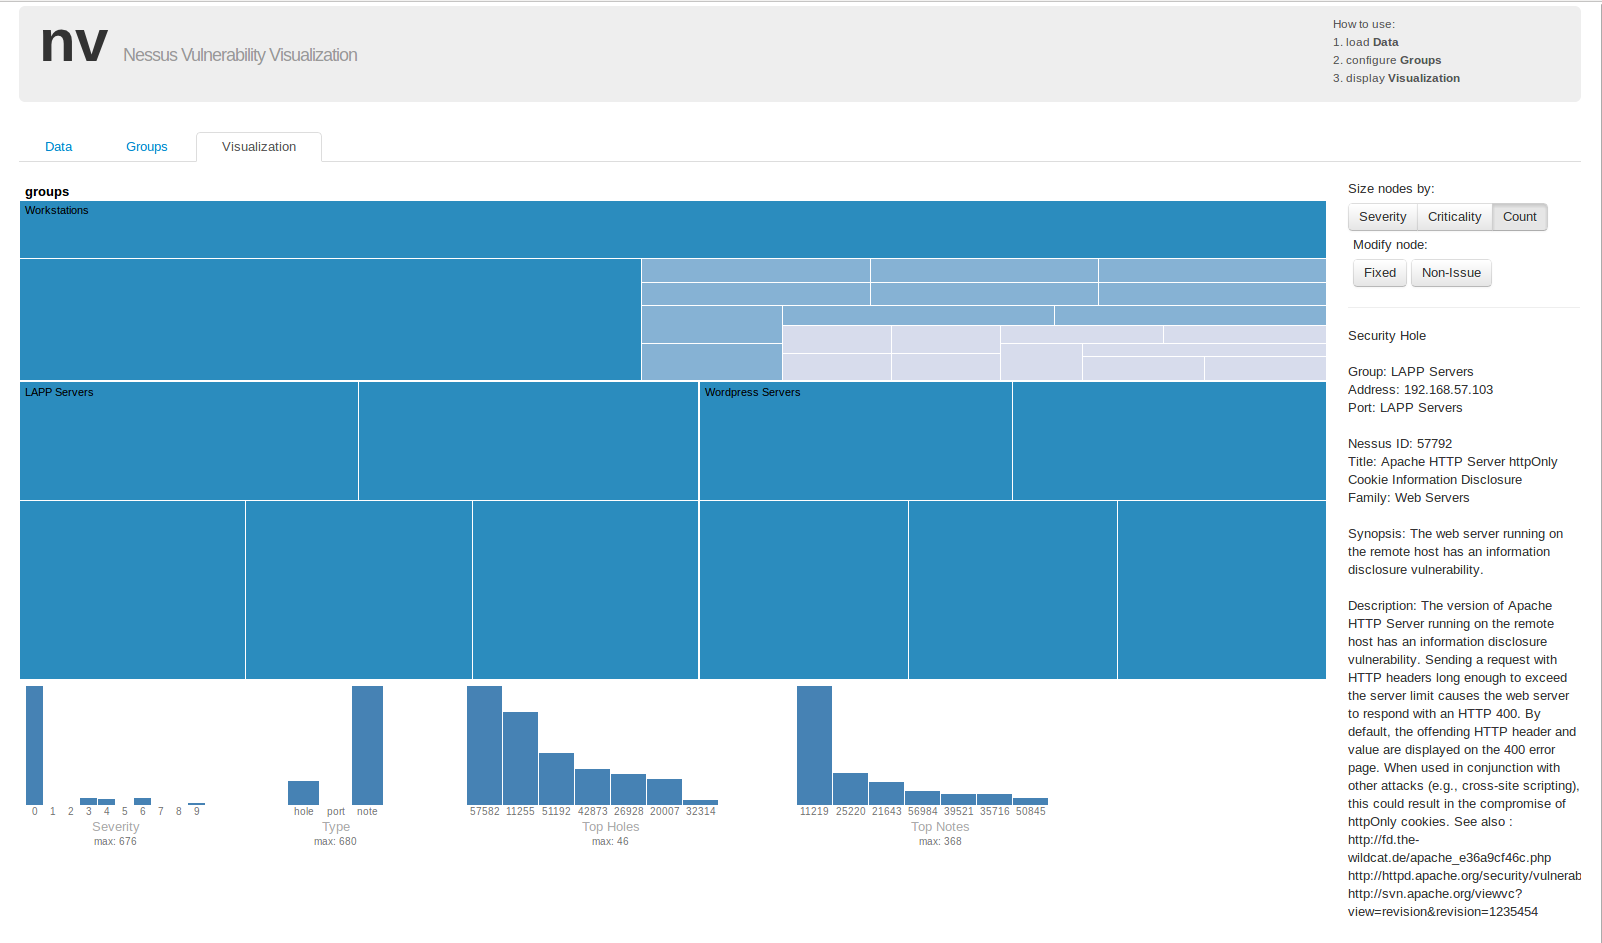
\includegraphics[width=0.5\textwidth]{../screenshots/final/SimGroupSingle}
  \caption{asdf}
\end{figure}

While in the criticality visualization mode the administrator's attention is
drawn to the large LAPP server node. The size is an indication of the
importance of the situation based on the number of security holes discovered,
the severity of the security holes discovered, and the assigned criticality of
the machines in the group. When the administrator zooms into the LAPP Server
node of the treemap they see that all five of the machines seem to be equally
at risk. To gain further insight, the administrator zooms into the node for a
specific machine where each node represents a port with an associated
vulnerability. At this specific port node the administrator can click on a
vulnerability ID and the tool will display information about the vulnerability
and potential solutions in the right-most panel of the tool. In this situation the LAPP servers all have the same
weak root password security hole. The system administrator will also find that
the Wordpress servers suffer from the same weak password vulnerability as the
LAPP servers.

%**Screenshot of zoomed in tree map can go here.**
%![Alt Text](screenshots/final/LAPPServerSimPort.png)
\begin{figure}
  \centering
  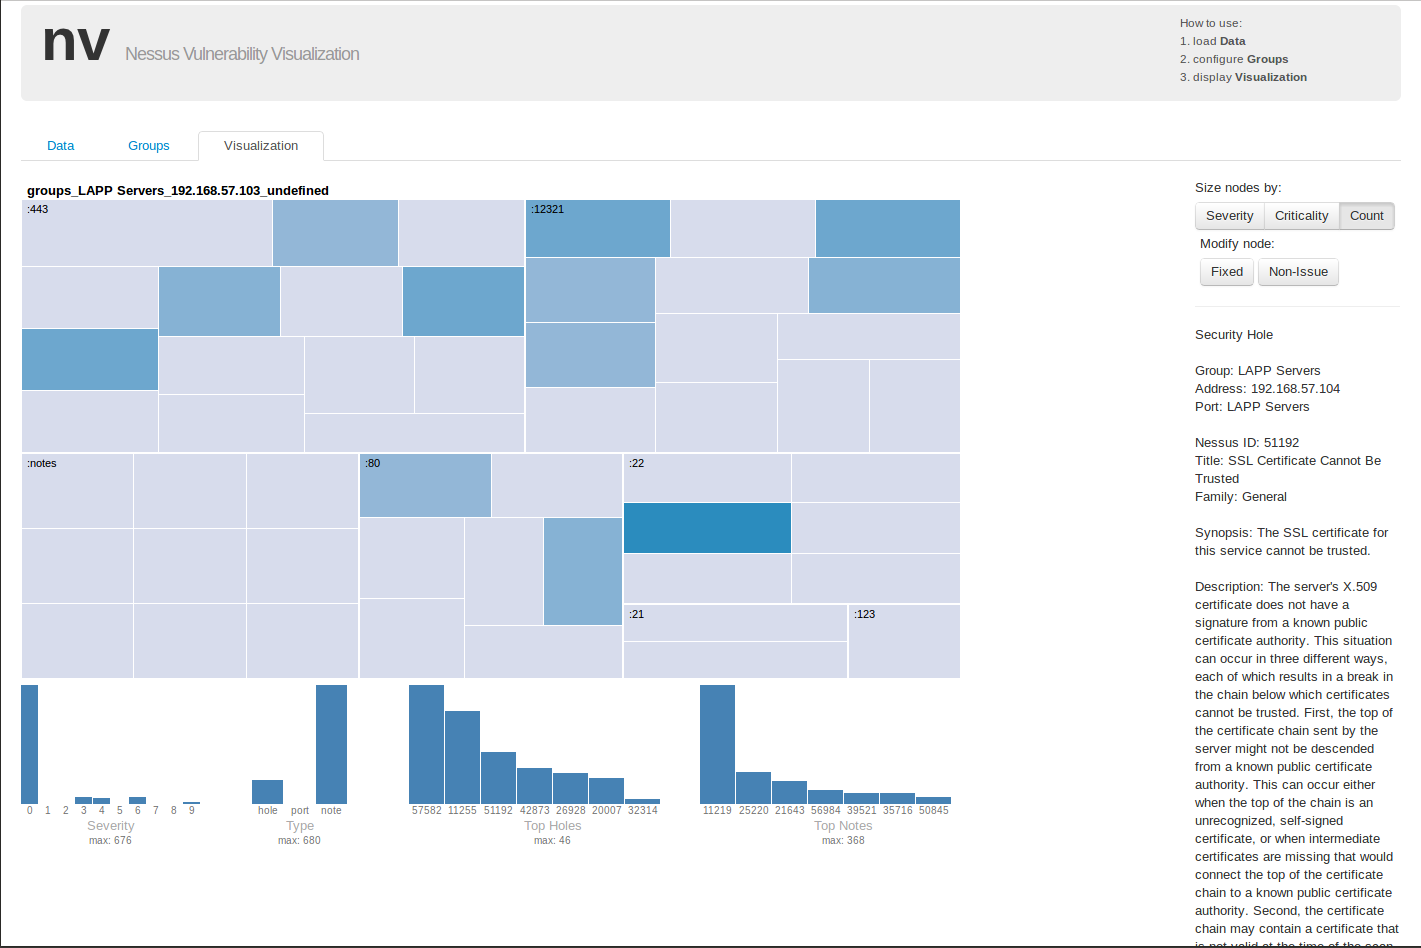
\includegraphics[width=0.5\textwidth]{../screenshots/final/LappServerSimPort}
  \caption{asdf}
\end{figure}

When the administrator zooms back out to the
group view and switches the visualization to severity mode, the workstation's
node grows bringing it into greater prominence. When the administrator
zooms into the workstation group they can see that two IP addresses have much
larger and darker nodes than any of the other workstations. If they zoom into
one of these IP addresses, they see that the most severe of the vulnerabilities
are associated with ports 445 and 80. The administrator can examine each port
node's child, seeing information about the specific vulnerabilities in the right-most
panel, discovering that the machine is running a poorly configured Apache
Web Server and that a Windows share that can be accessed through the network.

After further exploring their network, the administrator patches the most critical
vulnerabilities in the system. The Nessus Vulnerability Visualization system
provides functionality to compare two nbe files to show changes between two
vulnerability states, such as before and after applying patches. After patching
their system the administrator can rescan the network, then explore and see the
differences between the previous state and the newly patched system.
The Nessus Visualization System shows corrected
vulnerabilities in green, the remaining vulnerabilities in orange, and any new
vulnerabilities in pink. The system administrator can easily see that the
major workstations vulnerabilities have been patched. Zooming into the
workstation node the system administrator sees that while they were patching the most
severe vulnerabilities they inadvertently opened new vulnerabilities on the two
machines and did not address some of the vulnerabilities seen earlier.

\begin{center}
\begin{table*}
  \begin{tabular}{|l|l|l|l|l|l|}
    \hline Name:Criticality&IP Addresses&Time Period&Security Notes&Security Holes&Security Holes\\ \hline
    Workstations:2&192.168.56.x&Before Maintenance&680&18&18\\ \hline
    ~&~&After Maintenance&507&0&0\\ \hline
    LAPP Servers:9&192.168.57.x&Before Maintenance&205&5&5\\ \hline
    ~&~&After Maintenance&200&0&0\\ \hline
    Wordpress Servers:5&192.168.58.x&Before Maintenance&195&5&5\\ \hline
    ~&~&After Maintenance&195&0&0\\\hline
  \end{tabular}
  \caption{asdf}
\end{table*}
%**Screenshot of diff treemap.**
%![Alt Text](screenshots/final/SimDiffGroup.png)
\begin{figure}
  \centering
  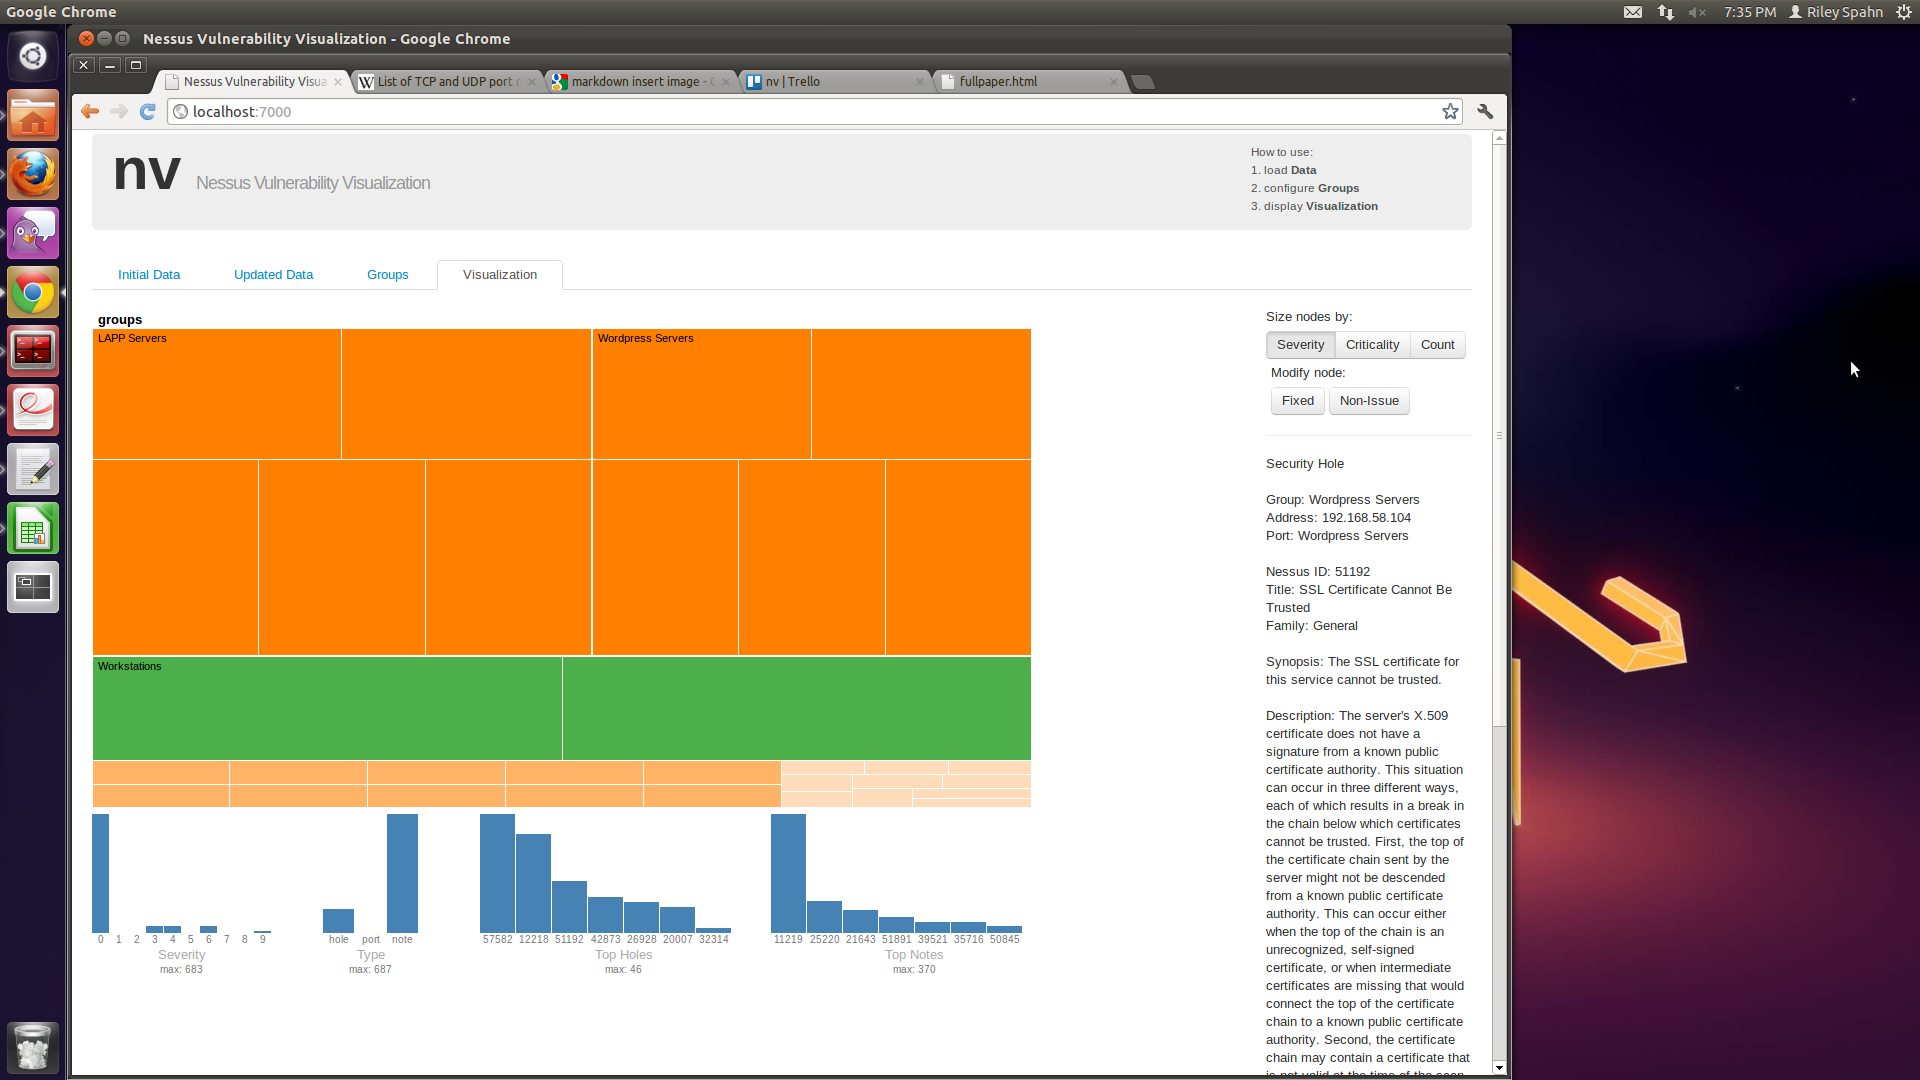
\includegraphics[width=0.5\textwidth]{../screenshots/final/SimDiffGroup}
  \caption{asdf}
\end{figure}
\end{center}

We simulated this use case using virtual machines (VM) communicating through a host-only
network. Using a host-only network allowed us to use Nessus from the host
to scan the VMs. We used one grouping of two different types of work station
and two groupings of similar servers. Both groups of servers were using Ubuntu 10.10 LTS.
Ten of the Ubuntu workstations were using Ubuntu 11.10 while the two workstations
with the massive number of vulnerabilities were using Ubuntu 8.04 with
purposely unpatched and misconfigured software.
The Fedora workstations were running Fedora 15.  We used the Metasploitable
virtual machine image to simulate the two vulnerable workstations before they
were upgraded to 11.10.

In this use case we did not patch all security notes that Nessus mentioned
because this would not be realistic for an actual system administrator. Instead,
the system administrator would only handle the most important vulnerabilities and
system updates. In this simulated use case we improved the weak root passwords
and corrected the poorly configured FTP server seen on the servers. We focused on updating
and correcting the two most vulnerable workstations by updating them to be the
same as the other ten Ubuntu workstations.



\subsection{Case Study 2: Static Vulnerability State Network }
To test visualizing a large static vulnerability state we use Nessus scan data from
the VAST Challenge 2011 (TODO cite). This data is from a simulated network for the
fictitious All Freight Corporation. The VAST Challenge gives us a large network
dataset to test how the Nessus Vulnerability Visualization scales to a large
data set that contains many vulnerabilities spread across a variety of machines and
groups. This data set has more than one
hundred-fifty unique IP addresses associated with various workstations in the
scan. The Nessus scan shows that numerous
machines on the network have some sort of security hole such as incorrectly
configured telnet client, a font driver that allows privilege escalation, and a
vulnerability in an outdated version of Microsoft Excel. The All Freight
Corporation has other machines and servers but they were not included in the
Nessus scan data.

%** Screenshot of over all **
%![Alt Text](screenshots/final/VastGroup.png)
\begin{figure}
  \centering
  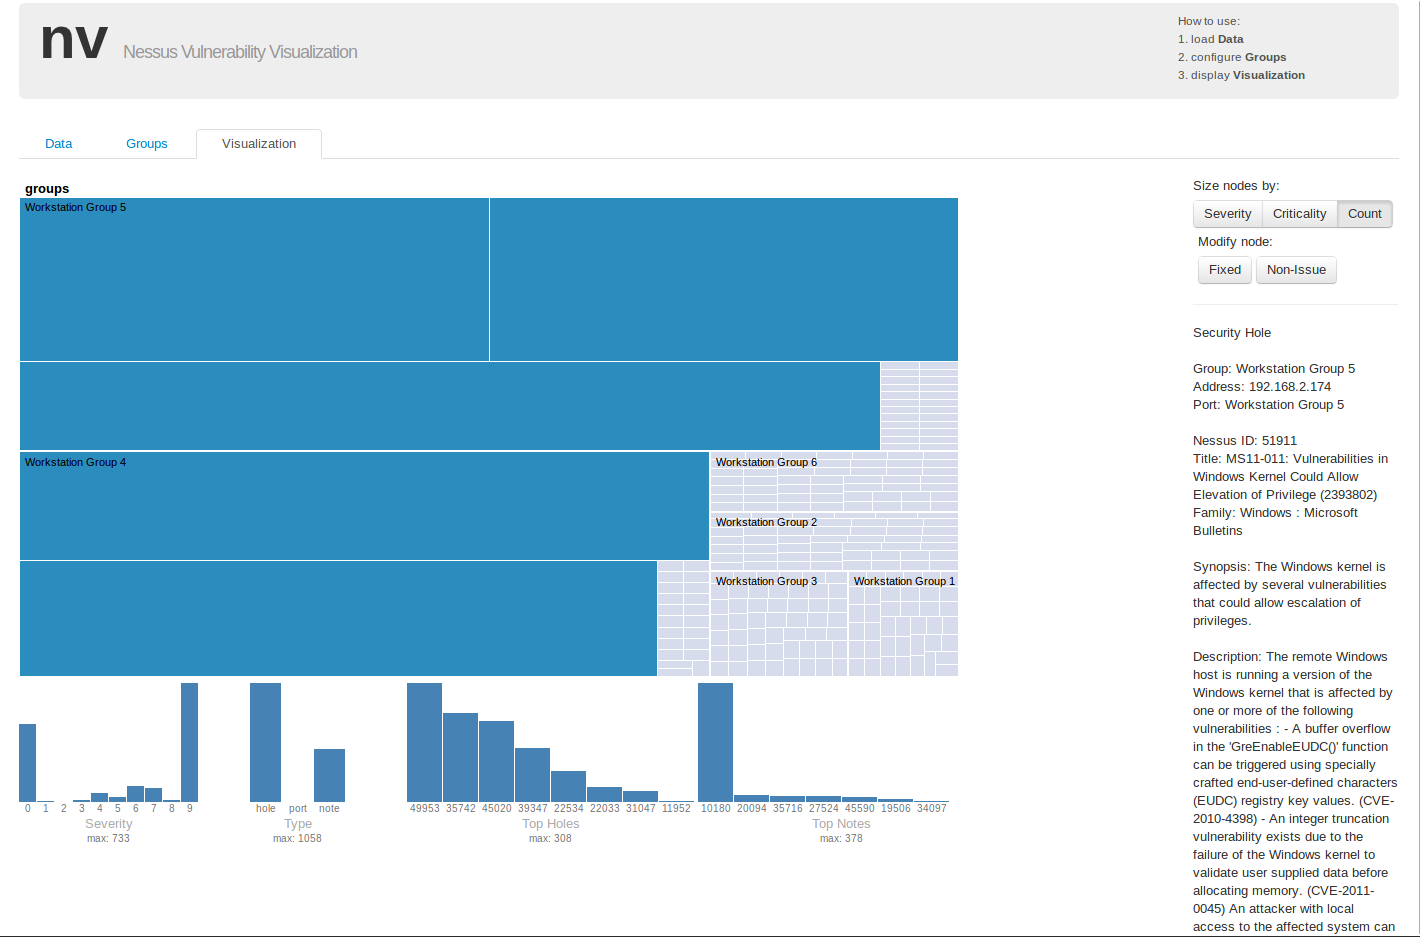
\includegraphics[width=0.5\textwidth]{../screenshots/final/VastGroup}
  \caption{asdf}
\end{figure}

We split the workstations into six groups with criticalities ranging from two to
nine.  The major security holes in the group are concentrated in group four with a
criticality of nine and in group five with a criticality of two.  When the
system administrator looks at the groups level on the tree map it is immediately
obvious where their attention is needed most. Groups four and five dominate the
treemap in all three visualization modes. When the system administrator zooms
into group four, they see that most of the vulnerabilities are located on two IP
addresses. When they select IP address 192.168.2.172, they see that nearly all of
the vulnerabilities are associated with port 445 and a Windows file sharing
program. The system administrator can also explore the other dominate IP address 192.168.2.171 and
see that this machines vulnerabilities come from port 139 and NetBIOS. The
Nessus Vulnerability Visualization system makes the most critical and most
severe vulnerabilities most prominent in the visualization. This
exploration allows the system administrator to easily discover vulnerabilities
in the system and prioritize repair accordingly. It also makes it easier to view large
networks because the IP addresses are aggregated into nodes that can be expanded to view
the individual IP addresses contained in that group.


%** Screen Shot of a zoomed in node **
%![Alt Text](screenshots/final/VASTWorkstationPort.png)
\begin{figure}
  \centering
  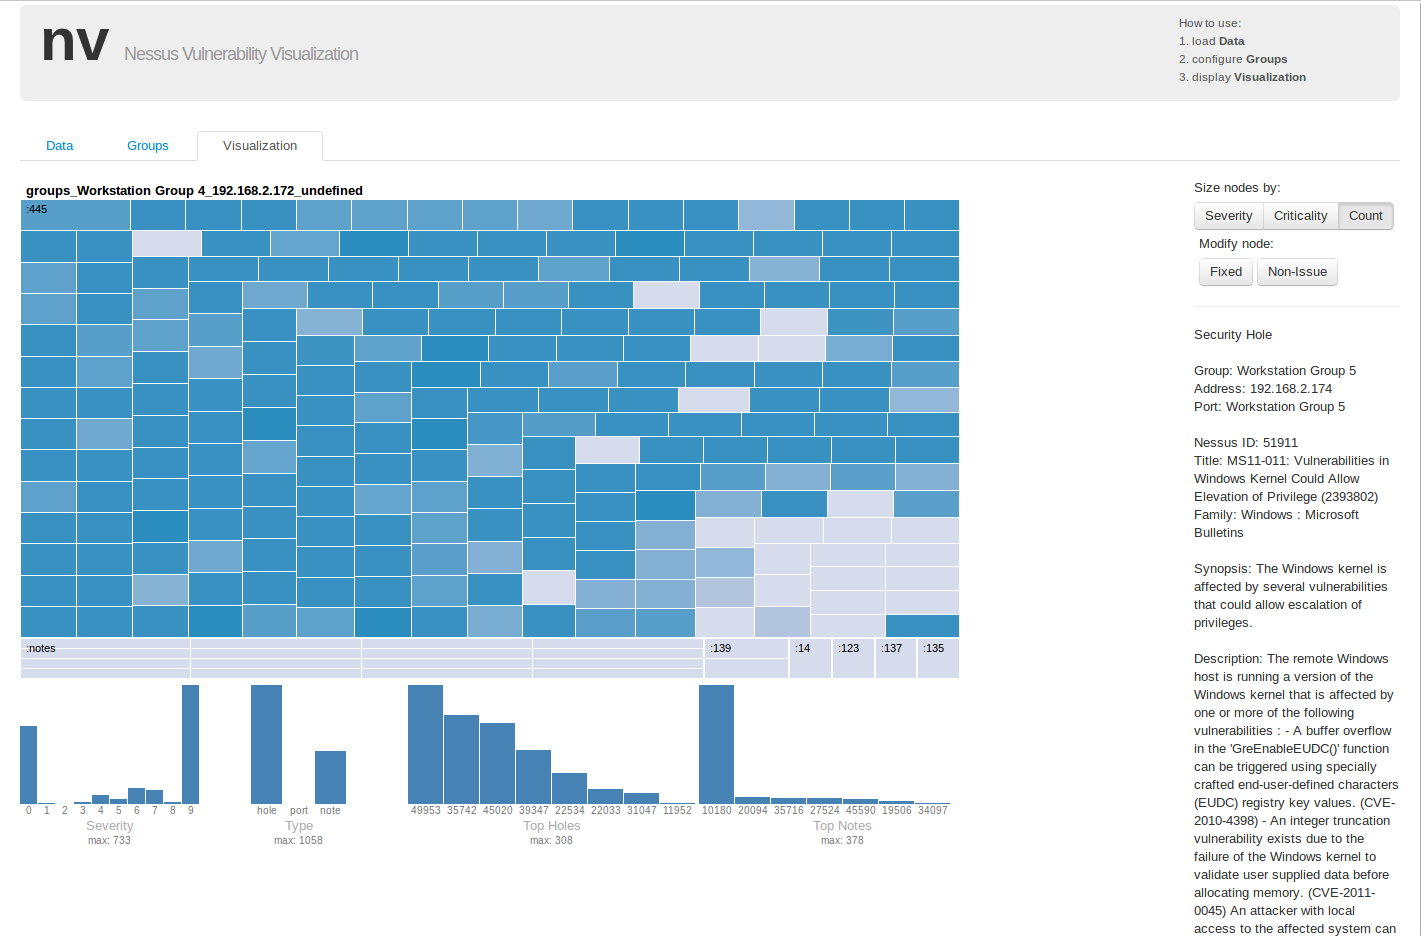
\includegraphics[width=0.5\textwidth]{../screenshots/final/VASTWorkstationPort}
  \caption{asdf}
\end{figure}

\section{Conclusion and Future Work}

We have introduced nv, a Nessus vulnerability visualization system.

Nv is designed to support sysadmins in the tasks of vulnerability discovery, analysis, and management through an interactive visualization.


%\end{document}  % This is where a 'short' article might terminate

\bibliographystyle{abbrv}
\bibliography{sigproc}  % sigproc.bib is the name of the Bibliography in this case

\subsection{References}
\end{document}

%%% Sample citation, table, conclusion
%\subsection{Citations}
%Citations to articles \cite{bowman:reasoning, clark:pct, braams:babel, herlihy:methodology},
%conference
%proceedings \cite{clark:pct} or books \cite{salas:calculus, Lamport:LaTeX} listed
%
%\begin{table*}
%\centering
%\caption{Some Typical Commands}
%\begin{tabular}{|c|c|l|} \hline
%Command&A Number&Comments\\ \hline
%\texttt{{\char'134}alignauthor} & 100& Author alignment\\ \hline
%\texttt{{\char'134}numberofauthors}& 200& Author enumeration\\ \hline
%\texttt{{\char'134}table}& 300 & For tables\\ \hline
%\texttt{{\char'134}table*}& 400& For wider tables\\ \hline\end{tabular}
%\end{table*}
%% end the environment with {table*}, NOTE not {table}!
%
%\begin{figure}
%\centering
%
\epsfig{file=fly.eps}
%\caption{A sample black and white graphic (.eps format).}
%\end{figure}


